\subsubsection{Teorijska nastava}
\label{subsubsec:prijava za nastavu}
\begin{itemize}
  \item \textbf{Kratak opis}: Kandidat koji se upisao u auto skolu pocinje sa pohadjanjem teorijske nastave u izabranoj grupi. Predavac evidentira prisustvo kandidata na casovima teorije koje on drzi.
  \item \textbf{Učesnici}:
    \begin{itemize}
    \item  Kandidat - korisnik sistema koji pohadja nastavu.
    \item  Predavac - korisnik koji drzi casove i evidentira prisustvo.
    \end{itemize}
  \item \textbf{Preduslovi}:
    \begin{itemize}
    \item  kandidat mora biti upisan u auto skolu.
    \item  kandidat mora biti rasporedjen u grupu kod predavaca.
    \item  kandidat je izmirio  prethodne troskove upisa.
    \item  predavac je zaduzen za grupu koju kandidati pohadjaju.
    \item  predavac je ulogovan na sistem.
    \item  sistem je dosutpan.
    \item  u sistemu ne postoji evidentiran cas za grupu u tekucem danu.
    \item  predavac  ima pristup internetu.
    \end{itemize}
  \item \textbf{Postuslovi}:
      \begin{itemize}
      \item Kandidat je evidentiran da je pohadjao nastavu.
      \item Predavac je evidnetirao odrzano predavanje.
      \end{itemize}
  \item \textbf{Osnovni tok}:
      \begin{enumerate}
        \item Predavac otvara stranicu za evidenciju prisustva korisnika.
        \item Predavac popunjava formular za zapocinjanje casa sa grupom.
        \item Predavac potvrdjuje da zapocinje cas sa grupom.
        \item Sistem prikazuje listu kandidata koji pohadjaju nastavu u toj grupi.
        \item Predavac evidentira prisustvo za svakog kandidata.
        \item Predavac zakljucuje evidenciju.
        \item Predavac zapocinje predavanje.
        \item Predavac nakon odrzanog cas zakljucuje cas.
        \item Sistem salje mail svim ucesnicima o uspeno zavrsenom casu i njihovom napretku.
      \end{enumerate}

  \item \textbf{Alternativni tokovi}:
      \begin{itemize}
        \item A1. \textbf{Neuspela validacija.}Ukoliku u koraku 2 sistem pronalazi neispravno polje formulara sistem obelezava polje koje treba ispraviti crvenom bojom, a ispod polja pise  uzrok neispravnosti. Nakon ponovnog ispravnog unosa podataka proces se nastavlja u koraku 3 osnovnog toka.s
      \end{itemize}
      
 \item \textbf{Dodatne informacije}:
      \begin{itemize}
        \item Polja formulara pri zapocinjanju cas su: Grupa, termin, cas.
      \end{itemize}
\end{itemize}

\begin{figure}[H]
  \begin{center}
      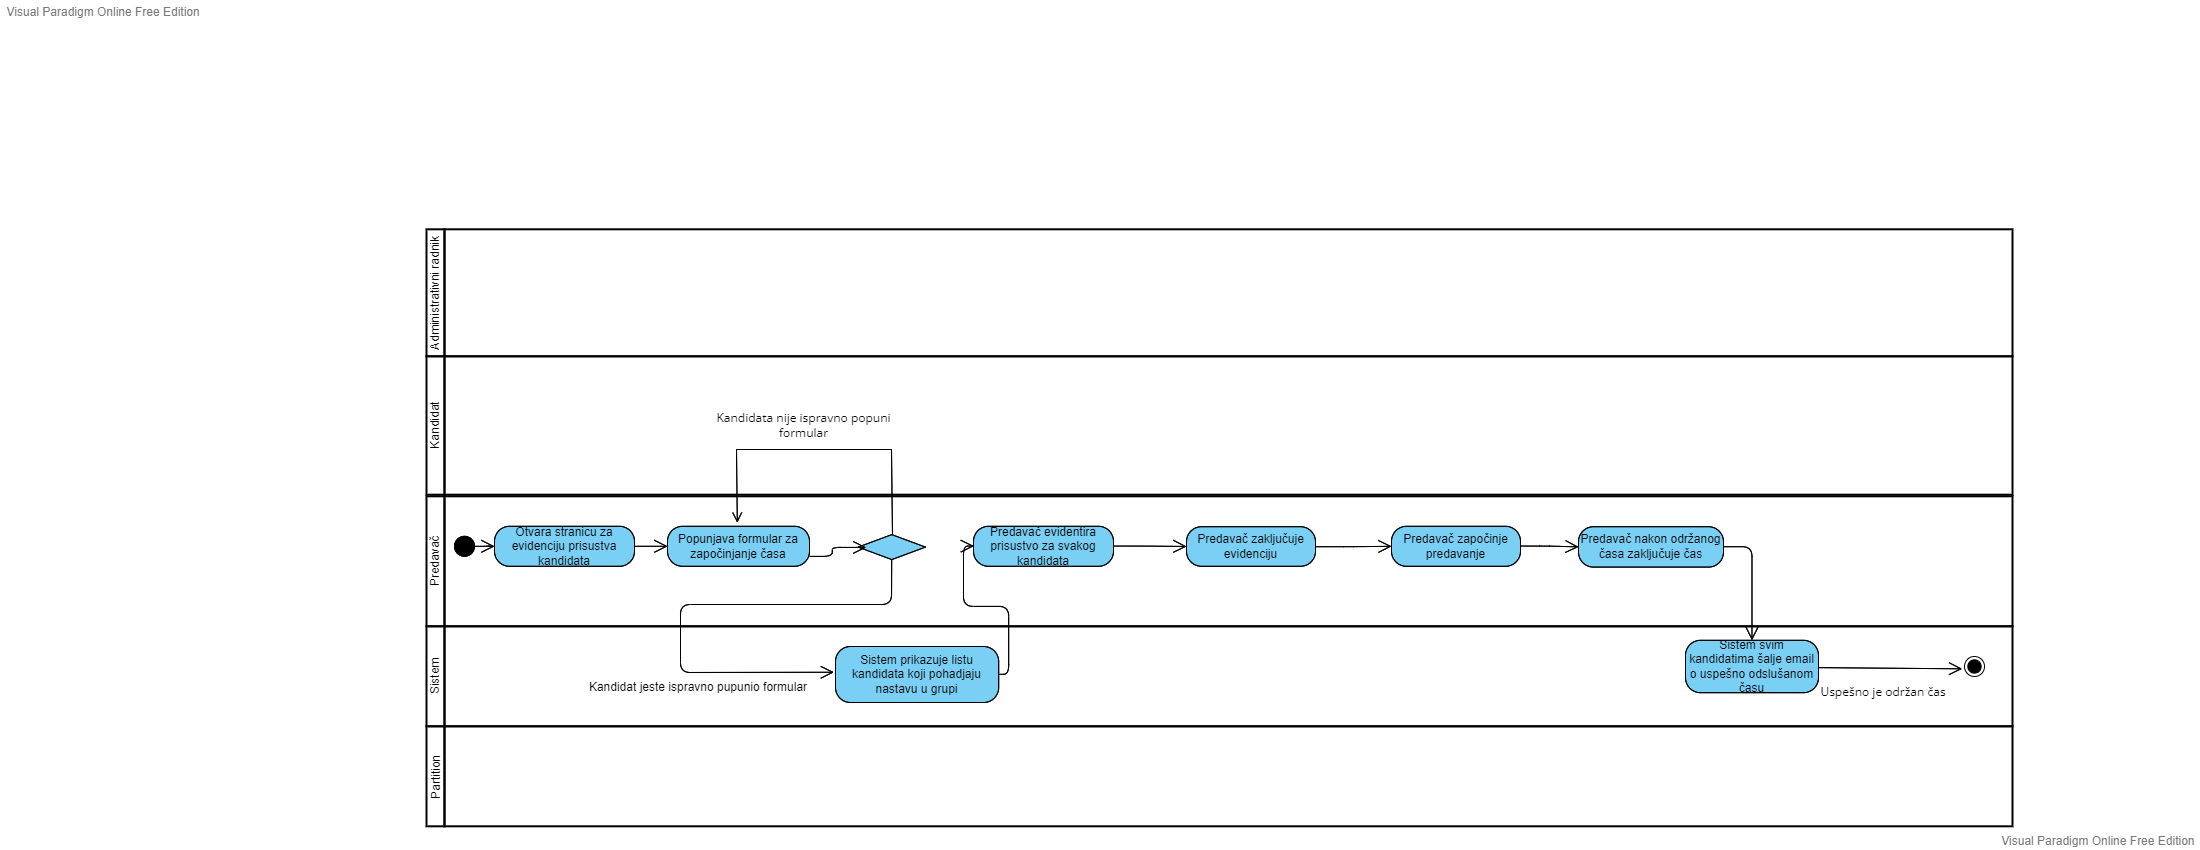
\includegraphics[width=140mm, height=70mm]{Diagrams/teorijska nastava dijagram.png}
  \end{center}
  \caption {Dijagram aktivnosti - teorijska nastava}
  \label{activity_diagram}

\end{figure}
